% --- IMPORTS ---
\documentclass[leqno]{article}
\usepackage{graphicx}
\usepackage{dsfont}
\usepackage{mathtools}
\usepackage{amssymb}
\usepackage{amsmath}
\usepackage{amsthm}
\usepackage{float}
\usepackage{ragged2e}
\usepackage{tensor}
\usepackage{fancyhdr}
\usepackage{empheq}
\usepackage[most]{tcolorbox}
\usepackage{enumitem}
\usepackage{dirtytalk}
\usepackage{marginnote}
\usepackage{microtype}
\usepackage[
  a4paper,
  left=0.8in,
  right=1in,
  top=1in,
  bottom=0.5in,
  headheight=14pt,
  headsep=0.4in
]{geometry}
\setlength{\parindent}{0cm}
% --- TikZ Packages ---
\usepackage{pgfplots}
\pgfplotsset{compat=1.18}
\usepgfplotslibrary{fillbetween, polar}
\usetikzlibrary{calc, positioning}
\usetikzlibrary{angles, quotes}
\usetikzlibrary{arrows.meta}
\usetikzlibrary{decorations.pathreplacing, decorations.markings}
\usetikzlibrary{patterns}
\usetikzlibrary{intersections}
% --- URL Packages ---
\usepackage[colorlinks=true,linkcolor=red,citecolor=magenta,urlcolor=black]{hyperref}%
\urlstyle{same}
% --- END OF IMPORTS ---

% --- CUSTOM COMMANDS ---
\RenewDocumentCommand{\marks}{o m}{%
  \IfValueTF{#1}%
    {\marginnote{\raggedright\textbf{[#2]}}[#1]}%
    {\marginnote{\raggedright\textbf{[#2]}}}%
}
\newcommand{\vspacerule}[2]{%
  \par\vspace*{#1}%
  \noindent\hrulefill\par
  \vspace*{#2}%
}
\definecolor{scarlet}{RGB}{205, 40, 75}
\newcommand{\questionitem}{%
  \item\phantomsection
  \addcontentsline{toc}{section}{Question \number\value{enumi}}%
}
\renewcommand{\contentsname}{Questions}
% --- END OF CUSTOM COMMANDS ---

% --- HEADER CONFIG ---
\pagestyle{fancy}
\fancyhead{}
\fancyfoot{}
\renewcommand{\headrulewidth}{0.9pt}
\lhead{\textit{Solutions} - Systems of Differential Equations}
\chead{}
\rhead{\href{https://danieljsmith.org}{danieljsmith.org}}
% --- END OF HEADER CONFIG ---

\begin{document}
\vspace*{20pt}
\tableofcontents
\newpage
\begin{enumerate}[
  label=\textbf{\arabic*.},
  leftmargin=*,
  topsep=0pt,
  partopsep=0pt,
  parsep=0pt
]

% ---- Question 1 ----
\questionitem

The functions $x$ and $y$ satisfy
\begin{align*}
\frac{\mathrm{d}x}{\mathrm{d}t}+\,\,\,y&=5x\\[5pt]
\frac{\mathrm{d}y}{\mathrm{d}t}+2y&=6x
\end{align*} \\
\begin{enumerate}[label=\textbf{(\alph*)}]
  \item Differentiate the first equation and eliminate $y$ to show that $x$ satisfies\\
  \[
  \frac{\mathrm{d}^2 x}{\mathrm{d}t^2}-3\frac{\mathrm{d}x}{\mathrm{d}t}-4x=0
  \]
  \marks[-30pt]{4}
  \item Given that $x=1$ and $y=3$ when $t=0$, find explicit expressions for $x$ and $y$ in terms of $t$. \marks{7} \\
\end{enumerate}

\vspace*{10pt}

\begin{tcolorbox}[colback=white, colframe=scarlet, title={\textbf{Solution}}, breakable, grow to left by=6mm, grow to right by=10mm]
\begin{enumerate}[label=\textbf{(\alph*)}]
  \item From
\[
\frac{\mathrm{d}x}{\mathrm{d}t}+y=5x
\]
we first rearrange to express $y$ in terms of $x$:
\[
y=5x-\frac{\mathrm{d}x}{\mathrm{d}t}
\]

Differentiate the first equation with respect to $t$:
\[
\frac{\mathrm{d}^2x}{\mathrm{d}t^2}+\frac{\mathrm{d}y}{\mathrm{d}t}=5\frac{\mathrm{d}x}{\mathrm{d}t}
\]

From the second equation,
\[
\frac{\mathrm{d}y}{\mathrm{d}t}+2y=6x
\]
so
\[
\frac{\mathrm{d}y}{\mathrm{d}t}=6x-2y
\]

Substitute this into the differentiated equation:
\begin{align*}
\frac{\mathrm{d}^2x}{\mathrm{d}t^2}+6x-2y&=5\frac{\mathrm{d}x}{\mathrm{d}t}
\end{align*}

Now substitute $y=5x-\dfrac{\mathrm{d}x}{\mathrm{d}t}$:
\begin{align*}
\frac{\mathrm{d}^2x}{\mathrm{d}t^2}+6x-2\left(5x-\frac{\mathrm{d}x}{\mathrm{d}t}\right)&=5\frac{\mathrm{d}x}{\mathrm{d}t} \\
\frac{\mathrm{d}^2x}{\mathrm{d}t^2}+6x-10x+2\frac{\mathrm{d}x}{\mathrm{d}t}&=5\frac{\mathrm{d}x}{\mathrm{d}t} \\
\frac{\mathrm{d}^2x}{\mathrm{d}t^2}-4x+2\frac{\mathrm{d}x}{\mathrm{d}t}-5\frac{\mathrm{d}x}{\mathrm{d}t}&=0 \\
\frac{\mathrm{d}^2x}{\mathrm{d}t^2}-3\frac{\mathrm{d}x}{\mathrm{d}t}-4x&=0
\end{align*}

Hence,
\[
\frac{\mathrm{d}^2x}{\mathrm{d}t^2}-3\frac{\mathrm{d}x}{\mathrm{d}t}-4x=0
\]

  \item We solve the differential equation found in part (a):
\[
\frac{\mathrm{d}^2x}{\mathrm{d}t^2}-3\frac{\mathrm{d}x}{\mathrm{d}t}-4x=0
\]

The auxiliary equation is
\[
\lambda^2-3\lambda-4=0
\]

Factorising,
\[
(\lambda-4)(\lambda+1)=0
\]

So the roots are $\lambda=4$ and $\lambda=-1$, giving
\[
x=A\mathrm{e}^{4t}+B\mathrm{e}^{-t}
\]

Differentiate:
\[
\frac{\mathrm{d}x}{\mathrm{d}t}=4A\mathrm{e}^{4t}-B\mathrm{e}^{-t}
\]

From the first original equation,
\[
\frac{\mathrm{d}x}{\mathrm{d}t}+y=5x
\]
so
\[
y=5x-\frac{\mathrm{d}x}{\mathrm{d}t}
\]

Substitute the expressions for $x$ and $\dfrac{\mathrm{d}x}{\mathrm{d}t}$:
\begin{align*}
y&=5\left(A\mathrm{e}^{4t}+B\mathrm{e}^{-t}\right)-\left(4A\mathrm{e}^{4t}-B\mathrm{e}^{-t}\right) \\
&=5A\mathrm{e}^{4t}+5B\mathrm{e}^{-t}-4A\mathrm{e}^{4t}+B\mathrm{e}^{-t} \\
&=A\mathrm{e}^{4t}+6B\mathrm{e}^{-t}
\end{align*}

Now use the initial conditions $x=1$ and $y=3$ when $t=0$.

From $x(0)=1$:
\begin{align*}
A+B&=1
\end{align*}

From $y(0)=3$:
\begin{align*}
A+6B&=3
\end{align*}

Subtract the first equation from the second:
\begin{align*}
(A+6B)-(A+B)&=3-1 \\
5B&=2 \\
B&=\frac{2}{5}
\end{align*}

Then
\begin{align*}
A+\frac{2}{5}&=1 \\
A&=\frac{3}{5}
\end{align*}

Substitute these values into $x$ and $y$:
\[
x=\frac{3}{5}\mathrm{e}^{4t}+\frac{2}{5}\mathrm{e}^{-t}
\]
and
\[
y=\frac{3}{5}\mathrm{e}^{4t}+\frac{12}{5}\mathrm{e}^{-t}
\]

Therefore the explicit expressions are
\[
x=\frac{3}{5}\mathrm{e}^{4t}+\frac{2}{5}\mathrm{e}^{-t},
\qquad
y=\frac{3}{5}\mathrm{e}^{4t}+\frac{12}{5}\mathrm{e}^{-t}
\]
\end{enumerate}
\end{tcolorbox}


\newpage

% ---- Question 2 ----
\questionitem

The functions $x$ and $y$ satisfy the simultaneous differential equations \\
\begin{align*}
\frac{\mathrm{d}x}{\mathrm{d}t}+y&=0\\[5pt]
\frac{\mathrm{d}y}{\mathrm{d}t}-x&=2e^{t}
\end{align*}
and when $t=0$, $x=0$ and $y=1$. \\

Solve the system, giving $x$ and $y$ explicitly in terms of $t$ \marks{11} \\

\vspace*{10pt}

\begin{tcolorbox}[colback=white, colframe=scarlet, title={\textbf{Solution}}, breakable, grow to left by=6mm, grow to right by=10mm]
From the first differential equation,
\[
\frac{\mathrm{d}x}{\mathrm{d}t}+y=0
\]
we have
\[
y=-\frac{\mathrm{d}x}{\mathrm{d}t}
\]

Differentiate this with respect to $t$:
\[
\frac{\mathrm{d}y}{\mathrm{d}t}=-\frac{\mathrm{d}^2x}{\mathrm{d}t^2}
\]

Now substitute $y$ and $\frac{\mathrm{d}y}{\mathrm{d}t}$ into
\[
\frac{\mathrm{d}y}{\mathrm{d}t}-x=2e^t
\]

This gives
\begin{align*}
-\frac{\mathrm{d}^2x}{\mathrm{d}t^2}-x&=2e^t \\
\frac{\mathrm{d}^2x}{\mathrm{d}t^2}+x&=-2e^t
\end{align*}

So we solve the second order linear equation
\[
\frac{\mathrm{d}^2x}{\mathrm{d}t^2}+x=-2e^t
\]

We also need initial conditions for $x$.

We are given
\[
x(0)=0
\]

Also, when $t=0$, the first equation gives
\begin{align*}
\frac{\mathrm{d}x}{\mathrm{d}t}+y&=0 \\
\frac{\mathrm{d}x}{\mathrm{d}t}+1&=0
\end{align*}
so
\[
\frac{\mathrm{d}x}{\mathrm{d}t}(0)=-1
\]

Now solve for $x$.

For the complementary function $x_c$, the auxiliary equation is
\[
\lambda^2+1=0
\]
so the roots are $\lambda=\pm i$.

Hence
\[
x_c=A\cos t+B\sin t
\]

For a particular integral $x_p$, since the right-hand side is $-2e^t$, try
\[
x_p=Ce^t
\]

Then
\[
\frac{\mathrm{d}^2x_p}{\mathrm{d}t^2}=Ce^t
\]

Substituting into the differential equation:
\begin{align*}
Ce^t+Ce^t&=-2e^t \\
2Ce^t&=-2e^t
\end{align*}
so
\[
C=-1
\]

Thus
\[
x_p=-e^t
\]

Therefore the general solution for $x$ is
\[
x=A\cos t+B\sin t-e^t
\]

Use the initial conditions.

First, $x(0)=0$:
\begin{align*}
A\cos 0+B\sin 0-e^0&=0 \\
A-1&=0
\end{align*}
so
\[
A=1
\]

Now differentiate $x$:
\[
\frac{\mathrm{d}x}{\mathrm{d}t}=-A\sin t+B\cos t-e^t
\]

Use $\frac{\mathrm{d}x}{\mathrm{d}t}(0)=-1$:
\begin{align*}
-A\sin 0+B\cos 0-e^0&=-1 \\
B-1&=-1
\end{align*}
so
\[
B=0
\]

Hence
\[
x=\cos t-e^t
\]

Now find $y$ from
\[
y=-\frac{\mathrm{d}x}{\mathrm{d}t}
\]

Since
\[
\frac{\mathrm{d}x}{\mathrm{d}t}=-\sin t-e^t
\]
it follows that
\[
y=\sin t+e^t
\]

So the required explicit solutions are
\[
x=\cos t-e^t, \qquad y=\sin t+e^t
\]
\end{tcolorbox}


\newpage

% ---- Question 3 ----
\questionitem

The functions $x$ and $y$ satisfy \\
\[
\begin{aligned}
\frac{\mathrm{d}x}{\mathrm{d}t} &= 3x+4y+7 \\[5pt]
\frac{\mathrm{d}y}{\mathrm{d}t} &= -x-y-1
\end{aligned}
\] \\

Given that $x=5$ and $y=-3$ when $t=0$, find $x$ and $y$ as functions of $t$ \marks{10} \\

\vspace*{10pt}

\begin{tcolorbox}[colback=white, colframe=scarlet, title={\textbf{Solution}}, breakable, grow to left by=6mm, grow to right by=10mm]
From the second differential equation,
\[
\frac{\mathrm{d}y}{\mathrm{d}t}=-x-y-1
\]
so
\[
x=-\frac{\mathrm{d}y}{\mathrm{d}t}-y-1
\]

Differentiate this to obtain an expression for \(\frac{\mathrm{d}x}{\mathrm{d}t}\):
\[
\frac{\mathrm{d}x}{\mathrm{d}t}=-\frac{\mathrm{d}^2y}{\mathrm{d}t^2}-\frac{\mathrm{d}y}{\mathrm{d}t}
\]

Now substitute both expressions into
\[
\frac{\mathrm{d}x}{\mathrm{d}t}=3x+4y+7
\]

This gives
\begin{align*}
-\frac{\mathrm{d}^2y}{\mathrm{d}t^2}-\frac{\mathrm{d}y}{\mathrm{d}t}
&=3\left(-\frac{\mathrm{d}y}{\mathrm{d}t}-y-1\right)+4y+7 \\
&=-3\frac{\mathrm{d}y}{\mathrm{d}t}-3y-3+4y+7 \\
&=-3\frac{\mathrm{d}y}{\mathrm{d}t}+y+4
\end{align*}

Rearranging,
\begin{align*}
-\frac{\mathrm{d}^2y}{\mathrm{d}t^2}-\frac{\mathrm{d}y}{\mathrm{d}t}
&=-3\frac{\mathrm{d}y}{\mathrm{d}t}+y+4 \\
-\frac{\mathrm{d}^2y}{\mathrm{d}t^2}+2\frac{\mathrm{d}y}{\mathrm{d}t}-y
&=4 \\
\frac{\mathrm{d}^2y}{\mathrm{d}t^2}-2\frac{\mathrm{d}y}{\mathrm{d}t}+y
&=-4
\end{align*}

We now solve this second-order linear differential equation.

The complementary function \(y_c\) satisfies the auxiliary equation
\[
\lambda^2-2\lambda+1=0
\]
so
\[
(\lambda-1)^2=0
\]

Hence
\[
y_c=(A+Bt)e^t
\]

For a particular integral \(y_p\), try a constant \(y_p=k\). Substituting into
\[
\frac{\mathrm{d}^2y}{\mathrm{d}t^2}-2\frac{\mathrm{d}y}{\mathrm{d}t}+y=-4
\]
gives
\[
0-0+k=-4
\]
so
\[
k=-4
\]

Therefore,
\[
y=(A+Bt)e^t-4
\]

Use the initial condition \(y(0)=-3\):
\begin{align*}
(A+0)e^0-4&=-3 \\
A-4&=-3 \\
A&=1
\end{align*}

So
\[
y=(1+Bt)e^t-4
\]

Now find \(x\) using
\[
x=-\frac{\mathrm{d}y}{\mathrm{d}t}-y-1
\]

First differentiate \(y\):
\begin{align*}
\frac{\mathrm{d}y}{\mathrm{d}t}
&=\frac{\mathrm{d}}{\mathrm{d}t}\left((A+Bt)e^t-4\right) \\
&=(A+Bt)e^t+Be^t \\
&=(A+Bt+B)e^t
\end{align*}

So
\begin{align*}
x
&=-(A+Bt+B)e^t-\left((A+Bt)e^t-4\right)-1 \\
&=-(2A+2Bt+B)e^t+3
\end{align*}

Now substitute \(A=1\):
\[
x=-(2+2Bt+B)e^t+3
\]

Use the initial condition \(x(0)=5\):
\begin{align*}
-(2+B)e^0+3&=5 \\
-(2+B)+3&=5 \\
1-B&=5 \\
B&=-4
\end{align*}

Substitute \(B=-4\) into the expressions for \(x\) and \(y\):
\begin{align*}
y(t)&=(1-4t)e^t-4 \\
x(t)&=-(2-8t-4)e^t+3 \\
&=(2+8t)e^t+3
\end{align*}

Therefore, the required functions are \(x(t)=(2+8t)e^t+3\) and \(y(t)=(1-4t)e^t-4\).
\end{tcolorbox}


\newpage

% ---- Question 4 ----
\questionitem

The functions $x$ and $y$ satisfy the system of differential equations
\begin{align*}
\frac{\mathrm{d}x}{\mathrm{d}t}&=x+2y-7 \\[5pt]
\frac{\mathrm{d}y}{\mathrm{d}t}&=2x+y-8
\end{align*}\\
\begin{enumerate}[label=\textbf{(\alph*)}]
  \item Find the stationary point of the system.\\ That is, find the values of $x$ and $y$ such that $\frac{\mathrm{d}x}{\mathrm{d}t}=0$ and $\frac{\mathrm{d}y}{\mathrm{d}t}=0$ \marks{2} \\
  \item Given that $x=4$ and $y=0$ when $t=0$, find the particular solutions for $x$ and $y$ in terms of $t$ \marks{8} \\
\end{enumerate}

\vspace*{10pt}

\begin{tcolorbox}[colback=white, colframe=scarlet, title={\textbf{Solution}}, breakable, grow to left by=6mm, grow to right by=10mm]
\begin{enumerate}[label=\textbf{(\alph*)}]
  \item At a stationary point,
  \[
  \frac{\mathrm{d}x}{\mathrm{d}t}=0
  \qquad \text{and} \qquad
  \frac{\mathrm{d}y}{\mathrm{d}t}=0
  \]

  So
  \begin{align*}
  x+2y-7&=0\\
  2x+y-8&=0
  \end{align*}

  Hence
  \[
  x+2y=7, \qquad 2x+y=8
  \]

  From the first equation,
  \[
  x=7-2y
  \]

  Substituting into the second equation:
  \begin{align*}
  2(7-2y)+y&=8\\
  14-4y+y&=8\\
  14-3y&=8\\
  3y&=6\\
  y&=2
  \end{align*}

  Then
  \[
  x=7-2(2)=3
  \]

  So the stationary point is $(3,2)$.

  \item Eliminate $y$ directly from the system.

  From
  \[
  \frac{\mathrm{d}x}{\mathrm{d}t}=x+2y-7
  \]
  we have
  \[
  2y=\frac{\mathrm{d}x}{\mathrm{d}t}-x+7
  \]

  Differentiate
  \[
  \frac{\mathrm{d}x}{\mathrm{d}t}=x+2y-7
  \]
  to obtain
  \[
  \frac{\mathrm{d}^2x}{\mathrm{d}t^2}
  =
  \frac{\mathrm{d}x}{\mathrm{d}t}
  +2\frac{\mathrm{d}y}{\mathrm{d}t}
  \]

  Now use
  \[
  \frac{\mathrm{d}y}{\mathrm{d}t}=2x+y-8
  \]
  so that
  \begin{align*}
  \frac{\mathrm{d}^2x}{\mathrm{d}t^2}
  &=\frac{\mathrm{d}x}{\mathrm{d}t}+2(2x+y-8)\\
  &=\frac{\mathrm{d}x}{\mathrm{d}t}+4x+2y-16
  \end{align*}

  Substitute
  \[
  2y=\frac{\mathrm{d}x}{\mathrm{d}t}-x+7
  \]
  to get
  \begin{align*}
  \frac{\mathrm{d}^2x}{\mathrm{d}t^2}
  &=\frac{\mathrm{d}x}{\mathrm{d}t}+4x+\left(\frac{\mathrm{d}x}{\mathrm{d}t}-x+7\right)-16\\
  &=2\frac{\mathrm{d}x}{\mathrm{d}t}+3x-9
  \end{align*}

  Therefore
  \[
  \frac{\mathrm{d}^2x}{\mathrm{d}t^2}-2\frac{\mathrm{d}x}{\mathrm{d}t}-3x=-9
  \]

  The auxiliary equation is
  \[
  \lambda^2-2\lambda-3=0
  \]

  Factorising:
  \[
  (\lambda-3)(\lambda+1)=0
  \]

  So the complementary function is
  \[
  x_c=A\mathrm{e}^{3t}+B\mathrm{e}^{-t}
  \]

  For a particular integral, try a constant value
  \[
  x_p=k
  \]

  Substituting into
  \[
  \frac{\mathrm{d}^2x}{\mathrm{d}t^2}-2\frac{\mathrm{d}x}{\mathrm{d}t}-3x=-9
  \]
  gives
  \[
  -3k=-9
  \]

  so
  \[
  k=3
  \]

  Hence
  \[
  x=x_c+x_p=A\mathrm{e}^{3t}+B\mathrm{e}^{-t}+3
  \]

  Now use the initial conditions.

  Since $x(0)=4$,
  \[
  A+B+3=4
  \]
  so
  \[
  A+B=1
  \]

  Also
  \[
  \frac{\mathrm{d}x}{\mathrm{d}t}=x+2y-7
  \]
  and when $t=0$,
  \[
  \left.\frac{\mathrm{d}x}{\mathrm{d}t}\right|_{t=0}=4+2(0)-7=-3
  \]

  But
  \[
  \frac{\mathrm{d}x}{\mathrm{d}t}=3A\mathrm{e}^{3t}-B\mathrm{e}^{-t}
  \]
  so at $t=0$,
  \[
  3A-B=-3
  \]

  Solving
  \[
  A+B=1,\qquad 3A-B=-3
  \]
  gives
  \[
  A=-\frac12,\qquad B=\frac32
  \]

  Therefore
  \[
  x=3-\frac12\mathrm{e}^{3t}+\frac32\mathrm{e}^{-t}
  \]

  Now find $y$ from
  \[
  2y=\frac{\mathrm{d}x}{\mathrm{d}t}-x+7
  \]

  Since
  \[
  \frac{\mathrm{d}x}{\mathrm{d}t}
  =-\frac32\mathrm{e}^{3t}-\frac32\mathrm{e}^{-t}
  \]
  we get
  \begin{align*}
  2y
  &=\left(-\frac32\mathrm{e}^{3t}-\frac32\mathrm{e}^{-t}\right)
    -\left(3-\frac12\mathrm{e}^{3t}+\frac32\mathrm{e}^{-t}\right)+7\\
  &=-\mathrm{e}^{3t}-3\mathrm{e}^{-t}+4
  \end{align*}

  Hence
  \[
  y=2-\frac12\mathrm{e}^{3t}-\frac32\mathrm{e}^{-t}
  \]

  Therefore the particular solutions are
  \[
  x=3-\frac12\mathrm{e}^{3t}+\frac32\mathrm{e}^{-t},
  \qquad
  y=2-\frac12\mathrm{e}^{3t}-\frac32\mathrm{e}^{-t}
  \]

\end{enumerate}
\end{tcolorbox}


\newpage

% ---- Question 5 ----
\questionitem

For $t\ge 0$, the functions $x=f(t)$ and $y=g(t)$ satisfy the coupled first-order differential equations. \\
\begin{align*}
\frac{\mathrm{d}x}{\mathrm{d}t}&=2x-y \\[5pt]
\frac{\mathrm{d}y}{\mathrm{d}t}&=x+2y
\end{align*} \\
Given that $x=1$ and $y=2$ when $t=0$, determine exact simplified expressions for $f(t)$ and $g(t)$ \marks{10} \\

\vspace*{10pt}

\begin{tcolorbox}[colback=white, colframe=scarlet, title={\textbf{Solution}}, breakable, grow to left by=6mm, grow to right by=10mm]
Starting with
\[
\frac{\mathrm{d}x}{\mathrm{d}t}=2x-y
\]
we first express \(y\) in terms of \(x\) and \(\frac{\mathrm{d}x}{\mathrm{d}t}\):
\[
y=2x-\frac{\mathrm{d}x}{\mathrm{d}t}
\]

Differentiate this with respect to \(t\):
\[
\frac{\mathrm{d}y}{\mathrm{d}t}=2\frac{\mathrm{d}x}{\mathrm{d}t}-\frac{\mathrm{d}^2x}{\mathrm{d}t^2}
\]

Now use the second differential equation:
\begin{align*}
\frac{\mathrm{d}y}{\mathrm{d}t}
&=x+2y\\
&=x+2\left(2x-\frac{\mathrm{d}x}{\mathrm{d}t}\right)\\
&=x+4x-2\frac{\mathrm{d}x}{\mathrm{d}t}\\
&=5x-2\frac{\mathrm{d}x}{\mathrm{d}t}
\end{align*}

Equating the two expressions for \(\frac{\mathrm{d}y}{\mathrm{d}t}\) gives
\begin{align*}
2\frac{\mathrm{d}x}{\mathrm{d}t}-\frac{\mathrm{d}^2x}{\mathrm{d}t^2}
&=5x-2\frac{\mathrm{d}x}{\mathrm{d}t}\\
-\frac{\mathrm{d}^2x}{\mathrm{d}t^2}+4\frac{\mathrm{d}x}{\mathrm{d}t}-5x&=0\\
\frac{\mathrm{d}^2x}{\mathrm{d}t^2}-4\frac{\mathrm{d}x}{\mathrm{d}t}+5x&=0
\end{align*}

So we solve the second-order linear differential equation
\[
\frac{\mathrm{d}^2x}{\mathrm{d}t^2}-4\frac{\mathrm{d}x}{\mathrm{d}t}+5x=0
\]

Its auxiliary equation is
\[
\lambda^2-4\lambda+5=0
\]

Solving,
\[
\lambda=\frac{4\pm\sqrt{16-20}}{2}=2\pm i
\]

Hence the complementary function is
\[
x=e^{2t}(A\cos t+B\sin t)
\]

Use the initial condition \(x(0)=1\):
\begin{align*}
x(0)&=e^0(A\cos 0+B\sin 0)\\
&=A
\end{align*}
so
\[
A=1
\]

To find \(B\), first find \(\frac{\mathrm{d}x}{\mathrm{d}t}\) at \(t=0\) from the original equation:
\begin{align*}
\left.\frac{\mathrm{d}x}{\mathrm{d}t}\right|_{t=0}
&=2x(0)-y(0)\\
&=2(1)-2\\
&=0
\end{align*}

Now differentiate
\[
x=e^{2t}(A\cos t+B\sin t)
\]

Using the product rule,
\begin{align*}
\frac{\mathrm{d}x}{\mathrm{d}t}
&=2e^{2t}(A\cos t+B\sin t)+e^{2t}(-A\sin t+B\cos t)\\
&=e^{2t}\bigl((2A+B)\cos t+(2B-A)\sin t\bigr)
\end{align*}

At \(t=0\),
\begin{align*}
0=\left.\frac{\mathrm{d}x}{\mathrm{d}t}\right|_{t=0}
&=e^0\bigl((2A+B)\cos 0+(2B-A)\sin 0\bigr)\\
&=2A+B
\end{align*}

Since \(A=1\),
\[
2(1)+B=0
\]
so
\[
B=-2
\]

Therefore
\[
x=e^{2t}(\cos t-2\sin t)
\]

Now find \(y\) using
\[
y=2x-\frac{\mathrm{d}x}{\mathrm{d}t}
\]

First differentiate \(x=e^{2t}(\cos t-2\sin t)\):
\begin{align*}
\frac{\mathrm{d}x}{\mathrm{d}t}
&=2e^{2t}(\cos t-2\sin t)+e^{2t}(-\sin t-2\cos t)\\
&=e^{2t}(2\cos t-4\sin t-\sin t-2\cos t)\\
&=-5e^{2t}\sin t
\end{align*}

So
\begin{align*}
y
&=2e^{2t}(\cos t-2\sin t)-\left(-5e^{2t}\sin t\right)\\
&=2e^{2t}\cos t-4e^{2t}\sin t+5e^{2t}\sin t\\
&=e^{2t}(2\cos t+\sin t)
\end{align*}

Hence the required functions are
\[
f(t)=e^{2t}(\cos t-2\sin t),\qquad g(t)=e^{2t}(2\cos t+\sin t)
\]
\end{tcolorbox}


\newpage

% ---- Question 6 ----
\questionitem

The functions $x$ and $y$ satisfy the simultaneous differential equations \\
\begin{align*}
\frac{\mathrm{d}x}{\mathrm{d}t}+y&=0\\[5pt]
\frac{\mathrm{d}y}{\mathrm{d}t}-x&=2
\end{align*}
and when $t=\dfrac{\pi}{2}$, $x=1$ and $y=2$. \\

Solve the system, giving $x$ and $y$ explicitly in terms of $t$ \marks{11} \\

\vspace*{20pt}

\begin{tcolorbox}[colback=white, colframe=scarlet, title={\textbf{Solution}}, breakable, grow to left by=6mm, grow to right by=10mm]
  From
  \[
  \frac{\mathrm{d}x}{\mathrm{d}t}+y=0
  \]
  we can write
  \[
  y=-\frac{\mathrm{d}x}{\mathrm{d}t}
  \]
  
  Differentiate this with respect to $t$:
  \[
  \frac{\mathrm{d}y}{\mathrm{d}t}=-\frac{\mathrm{d}^2x}{\mathrm{d}t^2}
  \]
  
  Now substitute into the second differential equation
  \[
  \frac{\mathrm{d}y}{\mathrm{d}t}-x=2
  \]
  to obtain
  \[
  -\frac{\mathrm{d}^2x}{\mathrm{d}t^2}-x=2
  \]
  so
  \[
  \frac{\mathrm{d}^2x}{\mathrm{d}t^2}+x=-2
  \]
  
  We now solve this second order differential equation.
  
  For the complementary function, solve
  \[
  \lambda^2+1=0
  \]
  so the roots are $\lambda=\pm \mathrm{i}$
  
  Hence
  \[
  x_c=A\cos t+B\sin t
  \]
  
  For a particular integral, since the right-hand side is a constant, try
  \[
  x_p=k
  \]
  Then
  \[
  0+k=-2
  \]
  so
  \[
  k=-2
  \]
  
  Therefore
  \[
  x=A\cos t+B\sin t-2
  \]
  
  Now use the initial conditions.
  
  When $t=\dfrac{\pi}{2}$, we are given that $x=1$, so
  \[
  1=A\cos \frac{\pi}{2}+B\sin \frac{\pi}{2}-2
  \]
  \[
  1=0+B-2
  \]
  \[
  B=3
  \]
  
  To find $A$, first differentiate $x$:
  \[
  \frac{\mathrm{d}x}{\mathrm{d}t}=-A\sin t+B\cos t
  \]
  
  Also, from
  \[
  \frac{\mathrm{d}x}{\mathrm{d}t}+y=0
  \]
  we have
  \[
  \frac{\mathrm{d}x}{\mathrm{d}t}=-y
  \]
  
  When $t=\dfrac{\pi}{2}$, $y=2$, so
  \[
  \frac{\mathrm{d}x}{\mathrm{d}t}=-2
  \]
  
  Substituting into the expression for $\dfrac{\mathrm{d}x}{\mathrm{d}t}$ gives
  \[
  -2=-A\sin \frac{\pi}{2}+B\cos \frac{\pi}{2}
  \]
  \[
  -2=-A(1)+3(0)
  \]
  \[
  A=2
  \]
  
  Hence
  \[
  x=2\cos t+3\sin t-2
  \]
  
  Finally, use
  \[
  y=-\frac{\mathrm{d}x}{\mathrm{d}t}
  \]
  
  Since
  \[
  \frac{\mathrm{d}x}{\mathrm{d}t}=-2\sin t+3\cos t
  \]
  it follows that
  \[
  y=2\sin t-3\cos t
  \]
  
  So the required solution is
  \[
  x=2\cos t+3\sin t-2, \qquad y=2\sin t-3\cos t
  \]
  
  A quick check:
  \[
  \frac{\mathrm{d}x}{\mathrm{d}t}+y=\left(-2\sin t+3\cos t\right)+\left(2\sin t-3\cos t\right)=0
  \]
  and
  \[
  \frac{\mathrm{d}y}{\mathrm{d}t}-x=\left(2\cos t+3\sin t\right)-\left(2\cos t+3\sin t-2\right)=2
  \]
  
  Also, when $t=\dfrac{\pi}{2}$,
  \[
  x=2\cos \frac{\pi}{2}+3\sin \frac{\pi}{2}-2=1
  \]
  \[
  y=2\sin \frac{\pi}{2}-3\cos \frac{\pi}{2}=2
  \]
  
  Therefore
  \[
  \boxed{x=2\cos t+3\sin t-2,\qquad y=2\sin t-3\cos t}
  \]
  \end{tcolorbox}


\newpage

% ---- Question 7 ----
\questionitem

An ecologist is studying the effect of introducing a population of weed-eating snails into a lake containing an invasive waterweed. During the first few months, a temporary pollutant also affects the snail population. \\

At time $t$ months, the amount of waterweed, $w$, and the number of snails, $s$, are modelled by the differential equations \\
\begin{align*}
\frac{\mathrm{d}w}{\mathrm{d}t}&=4w-s \\[5pt]
\frac{\mathrm{d}s}{\mathrm{d}t}&=6w-s-48e^{-t} \\
\end{align*}

\begin{enumerate}[label=\textbf{(\alph*)}]
  \item Show that
  \[\frac{\mathrm{d}^2 w}{\mathrm{d}t^2}-3\frac{\mathrm{d}w}{\mathrm{d}t}+2w=48e^{-t}\]
  \marks[-20pt]{3}
  \item Find a general solution for the amount of waterweed at time $t$ months \marks{6} \\
  \item Find a general solution for the number of snails at time $t$ months \marks{2} \\
\end{enumerate}
The model predicts that, at time $T$ months, the waterweed will have been eliminated. \\
Given that $w=30$ and $s=110$ when $t=0$ \\
\begin{enumerate}[label=\textbf{(\alph*)}, resume]
  \item Find the value of $T$, giving your answer to 3 decimal places \marks{6} \\
  \item Suggest one limitation of the model \marks{1} \\
\end{enumerate}

\vspace*{10pt}

\begin{tcolorbox}[colback=white, colframe=scarlet, title={\textbf{Solution}}, breakable, grow to left by=6mm, grow to right by=10mm]
\begin{enumerate}[label=\textbf{(\alph*)}]
  \item From
  \[
  \frac{\mathrm{d}w}{\mathrm{d}t}=4w-s
  \]
  we have
  \[
  s=4w-\frac{\mathrm{d}w}{\mathrm{d}t}
  \]

  Differentiate \(\dfrac{\mathrm{d}w}{\mathrm{d}t}=4w-s\) with respect to \(t\):
  \[
  \frac{\mathrm{d}^2w}{\mathrm{d}t^2}=4\frac{\mathrm{d}w}{\mathrm{d}t}-\frac{\mathrm{d}s}{\mathrm{d}t}
  \]

  Now use
  \[
  \frac{\mathrm{d}s}{\mathrm{d}t}=6w-s-48e^{-t}
  \]
  and substitute \(s=4w-\dfrac{\mathrm{d}w}{\mathrm{d}t}\):
  \begin{align*}
  \frac{\mathrm{d}s}{\mathrm{d}t}
  &=6w-\left(4w-\frac{\mathrm{d}w}{\mathrm{d}t}\right)-48e^{-t} \\
  &=2w+\frac{\mathrm{d}w}{\mathrm{d}t}-48e^{-t}
  \end{align*}

  So
  \begin{align*}
  \frac{\mathrm{d}^2w}{\mathrm{d}t^2}
  &=4\frac{\mathrm{d}w}{\mathrm{d}t}-\left(2w+\frac{\mathrm{d}w}{\mathrm{d}t}-48e^{-t}\right) \\
  &=3\frac{\mathrm{d}w}{\mathrm{d}t}-2w+48e^{-t}
  \end{align*}

  Hence
  \[
  \frac{\mathrm{d}^2w}{\mathrm{d}t^2}-3\frac{\mathrm{d}w}{\mathrm{d}t}+2w=48e^{-t}
  \]

  This is the required result.

  \item We solve
  \[
  \frac{\mathrm{d}^2w}{\mathrm{d}t^2}-3\frac{\mathrm{d}w}{\mathrm{d}t}+2w=48e^{-t}
  \]

  First find the complementary function \(w_c\) from
  \[
  \frac{\mathrm{d}^2w}{\mathrm{d}t^2}-3\frac{\mathrm{d}w}{\mathrm{d}t}+2w=0
  \]

  The auxiliary equation is
  \[
  \lambda^2-3\lambda+2=0
  \]

  Factorising,
  \[
  (\lambda-1)(\lambda-2)=0
  \]

  So the roots are \(\lambda=1\) and \(\lambda=2\), giving
  \[
  w_c=Ae^t+Be^{2t}
  \]

  For a particular integral \(w_p\), since the right-hand side is \(48e^{-t}\), try
  \[
  w_p=ke^{-t}
  \]

  Then
  \[
  \frac{\mathrm{d}w_p}{\mathrm{d}t}=-ke^{-t},
  \qquad
  \frac{\mathrm{d}^2w_p}{\mathrm{d}t^2}=ke^{-t}
  \]

  Substitute into the differential equation:
  \begin{align*}
  \frac{\mathrm{d}^2w_p}{\mathrm{d}t^2}-3\frac{\mathrm{d}w_p}{\mathrm{d}t}+2w_p
  &=ke^{-t}-3(-ke^{-t})+2ke^{-t} \\
  &=6ke^{-t}
  \end{align*}

  Comparing with \(48e^{-t}\),
  \[
  6k=48
  \]
  so
  \[
  k=8
  \]

  Therefore
  \[
  w_p=8e^{-t}
  \]

  Hence the general solution is
  \[
  w=w_c+w_p=Ae^t+Be^{2t}+8e^{-t}
  \]

  So the general solution for the waterweed is
  \[
  w=Ae^t+Be^{2t}+8e^{-t}
  \]

  \item From part (a),
  \[
  s=4w-\frac{\mathrm{d}w}{\mathrm{d}t}
  \]

  Using
  \[
  w=Ae^t+Be^{2t}+8e^{-t}
  \]
  we get
  \[
  \frac{\mathrm{d}w}{\mathrm{d}t}=Ae^t+2Be^{2t}-8e^{-t}
  \]

  So
  \begin{align*}
  s
  &=4\left(Ae^t+Be^{2t}+8e^{-t}\right)-\left(Ae^t+2Be^{2t}-8e^{-t}\right) \\
  &=3Ae^t+2Be^{2t}+40e^{-t}
  \end{align*}

  Therefore the general solution for the number of snails is
  \[
  s=3Ae^t+2Be^{2t}+40e^{-t}
  \]

  \item Use the initial conditions \(w=30\) and \(s=110\) when \(t=0\).

  From
  \[
  w=Ae^t+Be^{2t}+8e^{-t}
  \]
  when \(t=0\),
  \[
  30=A+B+8
  \]
  so
  \[
  A+B=22
  \]

  From
  \[
  s=3Ae^t+2Be^{2t}+40e^{-t}
  \]
  when \(t=0\),
  \[
  110=3A+2B+40
  \]
  so
  \[
  3A+2B=70
  \]

  Solve the simultaneous equations:
  \begin{align*}
  A+B&=22 \\
  3A+2B&=70
  \end{align*}

  Subtract \(2(A+B=22)\) from \(3A+2B=70\):
  \[
  A=26
  \]

  Then
  \[
  B=22-26=-4
  \]

  So
  \[
  w=26e^t-4e^{2t}+8e^{-t}
  \]

  The waterweed is eliminated when \(w=0\), so set \(w(T)=0\):
  \[
  26e^T-4e^{2T}+8e^{-T}=0
  \]

  Multiply through by \(e^T\):
  \[
  26e^{2T}-4e^{3T}+8=0
  \]

  Let
  \[
  x=e^T
  \]
  where \(x>0\). Then
  \[
  26x^2-4x^3+8=0
  \]

  Rearranging,
  \[
  2x^3-13x^2-4=0
  \]

  Solving this cubic numerically gives the positive root
  \[
  x\approx 6.547
  \]

  Therefore
  \[
  T=\ln(6.547)\approx 1.879
  \]

  So the value of \(T\) is
  \[
  T\approx 1.879 \text{ months}
  \]

  \item One limitation is that the model can predict negative values of \(w\) or \(s\), which is not realistic for populations.

  So a valid limitation is: the model can give impossible negative waterweed or snail populations.
\end{enumerate}
\end{tcolorbox}


\newpage

% ---- Question 8 ----
\questionitem

At the start of 2021, a survey began of the number of mature trees and saplings in a managed woodland. \\

At time $t$ years after the survey began, the number of mature trees, $m$, and the number of saplings, $s$, are modelled by the differential equations \\
\begin{align*}
\frac{\mathrm{d}m}{\mathrm{d}t}&=\frac{1}{4}s \\[5pt]
\frac{\mathrm{d}s}{\mathrm{d}t}&=-\frac{1}{20}m-\frac{1}{10}s \\
\end{align*}

\begin{enumerate}[label=\textbf{(\alph*)}]
  \item Show that
  \[\frac{\mathrm{d}^2 s}{\mathrm{d}t^2}+\frac{1}{10}\frac{\mathrm{d}s}{\mathrm{d}t}+\frac{1}{80}s=0\]
  \marks[-20pt]{3}
  \item Find a general solution for the number of saplings in the woodland at time $t$ years \marks{4} \\
  \item Hence find a general solution for the number of mature trees in the woodland at time $t$ years \marks{3} \\
\end{enumerate}
At the start of 2021 there were $20$ mature trees and $20$ saplings. \\
\begin{enumerate}[label=\textbf{(\alph*)}, resume]
  \item \begin{enumerate}[label=(\roman*)]
    \item According to this model, find the first value of $t$ for which no saplings remain, and state the year.
    \item According to this model, how many mature trees are there at that time?
    \item Use your answers to parts (i) and (ii) to comment on the suitability of the model.
  \end{enumerate}
  \marks[-10pt]{7} 
\end{enumerate}

\vspace*{10pt}

\begin{tcolorbox}[colback=white, colframe=scarlet, title={\textbf{Solution}}, breakable, grow to left by=6mm, grow to right by=10mm]
\begin{enumerate}[label=\textbf{(\alph*)}]
  \item Differentiate the equation for $\dfrac{\mathrm{d}s}{\mathrm{d}t}$ with respect to $t$:
  \begin{align*}
  \frac{\mathrm{d}^2s}{\mathrm{d}t^2}
  &= -\frac{1}{20}\frac{\mathrm{d}m}{\mathrm{d}t}-\frac{1}{10}\frac{\mathrm{d}s}{\mathrm{d}t}
  \end{align*}
  Using
  \[
  \frac{\mathrm{d}m}{\mathrm{d}t}=\frac14 s
  \]
  gives
  \begin{align*}
  \frac{\mathrm{d}^2s}{\mathrm{d}t^2}
  &= -\frac{1}{20}\left(\frac14 s\right)-\frac{1}{10}\frac{\mathrm{d}s}{\mathrm{d}t} \\
  &= -\frac{1}{80}s-\frac{1}{10}\frac{\mathrm{d}s}{\mathrm{d}t}
  \end{align*}
  Rearranging,
  \[
  \frac{\mathrm{d}^2s}{\mathrm{d}t^2}+\frac{1}{10}\frac{\mathrm{d}s}{\mathrm{d}t}+\frac{1}{80}s=0
  \]
  Hence the required equation is shown.

  \item From part (a), we solve
  \[
  \frac{\mathrm{d}^2s}{\mathrm{d}t^2}+\frac{1}{10}\frac{\mathrm{d}s}{\mathrm{d}t}+\frac{1}{80}s=0
  \]
  The auxiliary equation is
  \[
  \lambda^2+\frac{1}{10}\lambda+\frac{1}{80}=0
  \]
  Multiplying through by $80$,
  \[
  80\lambda^2+8\lambda+1=0
  \]
  Using the quadratic formula,
  \begin{align*}
  \lambda
  &= \frac{-8\pm\sqrt{8^2-4(80)(1)}}{160} \\
  &= \frac{-8\pm\sqrt{64-320}}{160} \\
  &= \frac{-8\pm\sqrt{-256}}{160} \\
  &= \frac{-8\pm 16\mathrm{i}}{160} \\
  &= -\frac{1}{20}\pm\frac{1}{10}\mathrm{i}
  \end{align*}
  Therefore the general solution is
  \[
  s=e^{-t/20}\left(A\cos\frac{t}{10}+B\sin\frac{t}{10}\right)
  \]
  So a general solution for the number of saplings is
  \[
  s=e^{-t/20}\left(A\cos\frac{t}{10}+B\sin\frac{t}{10}\right)
  \]

  \item Use
  \[
  \frac{\mathrm{d}s}{\mathrm{d}t}=-\frac{1}{20}m-\frac{1}{10}s
  \]
  Rearranging for $m$,
  \[
  m=-20\left(\frac{\mathrm{d}s}{\mathrm{d}t}+\frac{1}{10}s\right)
  \]
  Let $\theta=\dfrac{t}{10}$. From part (b),
  \[
  s=e^{-t/20}(A\cos\theta+B\sin\theta)
  \]
  Differentiate:
  \begin{align*}
  \frac{\mathrm{d}s}{\mathrm{d}t}
  &= -\frac{1}{20}e^{-t/20}(A\cos\theta+B\sin\theta)
   +e^{-t/20}\left(-\frac{A}{10}\sin\theta+\frac{B}{10}\cos\theta\right) \\
  &= e^{-t/20}\left[\left(\frac{B}{10}-\frac{A}{20}\right)\cos\theta
  +\left(-\frac{A}{10}-\frac{B}{20}\right)\sin\theta\right]
  \end{align*}
  Now substitute into the expression for $m$:
  \begin{align*}
  m
  &= -20\left(\frac{\mathrm{d}s}{\mathrm{d}t}+\frac{1}{10}s\right) \\
  &= -20e^{-t/20}\Bigg[\left(\frac{B}{10}-\frac{A}{20}+\frac{A}{10}\right)\cos\theta
  +\left(-\frac{A}{10}-\frac{B}{20}+\frac{B}{10}\right)\sin\theta\Bigg] \\
  &= -20e^{-t/20}\left[\left(\frac{A+2B}{20}\right)\cos\theta
  +\left(\frac{-2A+B}{20}\right)\sin\theta\right] \\
  &= e^{-t/20}\left[(-A-2B)\cos\theta+(2A-B)\sin\theta\right]
  \end{align*}
  Hence a general solution for the number of mature trees is
  \[
  m=e^{-t/20}\left[(-A-2B)\cos\frac{t}{10}+(2A-B)\sin\frac{t}{10}\right]
  \]

  \item \begin{enumerate}[label=(\roman*)]
    \item Use the initial conditions $s(0)=20$ and $m(0)=20$.

    From the formula for $s$,
    \begin{align*}
    s(0)&=A=20
    \end{align*}
    so $A=20$.

    From the formula for $m$,
    \begin{align*}
    m(0)&=-A-2B=20 \\
    -20-2B&=20 \\
    -2B&=40 \\
    B&=-20
    \end{align*}
    Therefore
    \[
    s=20e^{-t/20}\left(\cos\frac{t}{10}-\sin\frac{t}{10}\right)
    \]
    To find when no saplings remain, set $s=0$:
    \begin{align*}
    20e^{-t/20}\left(\cos\frac{t}{10}-\sin\frac{t}{10}\right)&=0
    \end{align*}
    Since $20e^{-t/20}\neq 0$, we need
    \begin{align*}
    \cos\frac{t}{10}-\sin\frac{t}{10}&=0 \\
    \tan\frac{t}{10}&=1
    \end{align*}
    The first positive solution is
    \[
    \frac{t}{10}=\frac{\pi}{4}
    \]
    so
    \[
    t=\frac{5\pi}{2}\approx 7.85
    \]
    This is about $7.85$ years after the start of 2021, so the year is 2028.

    The first value of $t$ is $\displaystyle \frac{5\pi}{2}$ years, so the year is 2028.

    \item Substituting $A=20$ and $B=-20$ into the formula for $m$,
    \[
    m=20e^{-t/20}\left(\cos\frac{t}{10}+3\sin\frac{t}{10}\right)
    \]
    At $t=\dfrac{5\pi}{2}$,
    \begin{align*}
    m
    &= 20e^{-(5\pi/2)/20}\left(\cos\frac{\pi}{4}+3\sin\frac{\pi}{4}\right) \\
    &= 20e^{-\pi/8}\left(\frac{1}{\sqrt{2}}+\frac{3}{\sqrt{2}}\right) \\
    &= 20e^{-\pi/8}\left(\frac{4}{\sqrt{2}}\right) \\
    &= 40\sqrt{2}\,e^{-\pi/8} \\
    &\approx 38.2
    \end{align*}
    So the model predicts about $38.2$ mature trees at that time.

    \item This model is not suitable beyond that time, because after $t=\dfrac{5\pi}{2}$ it gives $s<0$, meaning a negative number of saplings, which is impossible.

    Also, at $t=\dfrac{5\pi}{2}$ it predicts about $38.2$ mature trees, but numbers of trees should be whole numbers.

    Therefore the model is only reasonable for a limited time interval and is unsuitable in the longer term.
  \end{enumerate}
\end{enumerate}
\end{tcolorbox}


\newpage

% ---- Question 9 ----
\questionitem

\begin{figure}[H]
    \centering
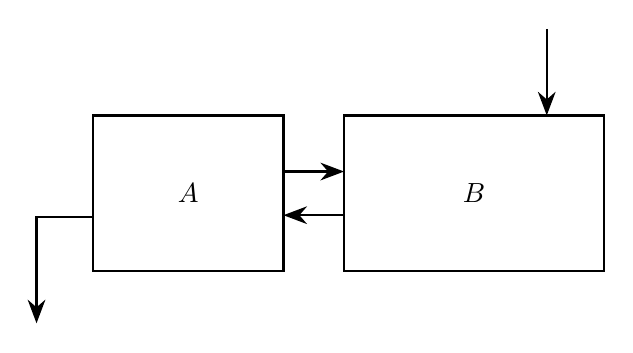
\begin{tikzpicture}[scale=1.1]
\def\aw{2.2}
\def\bw{3.0}
\def\th{1.8}
\def\gap{0.7}

\coordinate (A1) at (0,0);
\coordinate (A2) at (\aw,\th);
\coordinate (B1) at (\aw+\gap,0);
\coordinate (B2) at ({\aw+\gap+\bw},\th);

\draw[thick] (A1) rectangle (A2);
\draw[thick] (B1) rectangle (B2);

\node at ($(A1)!0.5!(A2)$) {$A$};
\node at ($(B1)!0.5!(B2)$) {$B$};

\coordinate (In1) at ({\aw+\gap+0.78*\bw},{\th+1});
\coordinate (In2) at ({\aw+\gap+0.78*\bw},\th);
\draw[thick,-{Stealth[length=3mm]}] (In1) -- (In2);

\coordinate (AB1) at (\aw,{0.64*\th});
\coordinate (AB2) at (\aw+\gap,{0.64*\th});
\draw[thick,-{Stealth[length=3mm]}] (AB1) -- (AB2);

\coordinate (BA1) at (\aw+\gap,{0.36*\th});
\coordinate (BA2) at (\aw,{0.36*\th});
\draw[thick,-{Stealth[length=3mm]}] (BA1) -- (BA2);

\coordinate (Out1) at (0,{0.35*\th});
\coordinate (Out2) at (-0.65,{0.35*\th});
\coordinate (Out3) at (-0.65,-0.6);
\draw[thick,-{Stealth[length=3mm]}] (Out1) -- (Out2) -- (Out3);
\end{tikzpicture}
\end{figure}

\vspace*{10pt}

A treatment system consists of two well-stirred tanks, $A$ and $B$. Tank $A$ has capacity 300 litres and tank $B$ has capacity 500 litres. \\

At time $t=0$, tank $A$ is full and contains 300 grams of salt, while tank $B$ is full and contains 1200 grams of salt. \\

When $t>0$, liquid flows in the following ways: \\
\begin{itemize}
  \item Brine with a salt concentration of $\mu$ grams per litre flows into tank $B$ at a constant rate
  \item Liquid flows from tank $A$ to tank $B$ at a rate of $3$ litres per minute
  \item Liquid flows from tank $B$ to tank $A$ at a rate of $r$ litres per minute
  \item Liquid flows out of tank $A$ through a waste pipe
  \item The amount of liquid in tank $A$ remains at $300$ litres and the amount of liquid in tank $B$ remains at $500$ litres \\
\end{itemize}
At time $t$ minutes ($t\ge 0$) there are $x$ grams of salt in tank $A$ and $y$ grams of salt in tank $B$. \\

This system is represented by the coupled differential equations

\begin{align*}
\dfrac{\mathrm{d}x}{\mathrm{d}t} & =  -\dfrac{1}{20}x+\dfrac{3}{100}y\\[6pt]
\dfrac{\mathrm{d}y}{\mathrm{d}t} & =  \dfrac{1}{100}x-\dfrac{3}{100}y + 24
\end{align*}
\\
\begin{enumerate}[label=\textbf{(\alph*)}]
  \item Find the value of $r$ \marks{2} \\
  \item Show that $\mu=2$ \marks{3} \\
  \item Solve the coupled differential equations to find both $x$ and $y$ in terms of $t$ \marks{9} \\
\end{enumerate}

\vspace*{10pt}

\begin{tcolorbox}[colback=white, colframe=scarlet, title={\textbf{Solution}}, breakable, grow to left by=6mm, grow to right by=10mm]
\begin{enumerate}[label=\textbf{(\alph*)}]
  \item Since the tanks are well stirred, the salt concentrations are
\[
\frac{x}{300}\text{ g L}^{-1} \quad \text{in tank }A,
\qquad
\frac{y}{500}\text{ g L}^{-1} \quad \text{in tank }B
\]
Let the waste outflow from tank $A$ be $w$ L min$^{-1}$. Since the volume of tank $A$ remains constant,
\[
r = 3 + w
\]
so the total outflow from tank $A$ is $r$ L min$^{-1}$.

Hence the salt balance for tank $A$ is
\[
\frac{\mathrm{d}x}{\mathrm{d}t}=\frac{r}{500}y-\frac{r}{300}x
\]
Comparing this with
\[
\frac{\mathrm{d}x}{\mathrm{d}t}=-\frac{1}{20}x+\frac{3}{100}y
\]
gives
\[
\frac{r}{300}=\frac{1}{20}
\]
so
\[
r=15
\]

Therefore $r=15$ litres per minute.

  \item Let the external inflow to tank $B$ be $q$ L min$^{-1}$. Since the volume of tank $B$ remains constant,
\[
q+3=r
\]
Using $r=15$ from part (a),
\[
q=15-3=12
\]

Now write the salt balance for tank $B$.

External inflow contributes salt at rate $12\mu$ g min$^{-1}$, inflow from $A$ contributes
\[
3\cdot \frac{x}{300}=\frac{x}{100}
\]
and outflow from $B$ to $A$ removes salt at rate
\[
15\cdot \frac{y}{500}=\frac{3y}{100}
\]

So
\[
\frac{\mathrm{d}y}{\mathrm{d}t}=12\mu+\frac{x}{100}-\frac{3y}{100}
\]
Comparing with the given equation
\[
\frac{\mathrm{d}y}{\mathrm{d}t}=24+\frac{x}{100}-\frac{3y}{100}
\]
we get
\[
12\mu=24
\]
and therefore
\[
\mu=2
\]

Therefore $\mu=2\text{ g L}^{-1}$.

  \item To solve the system, eliminate $y$.

From equation (1),
\begin{align*}
\frac{\mathrm{d}x}{\mathrm{d}t} &= -\frac{1}{20}x+\frac{3}{100}y \\
100\frac{\mathrm{d}x}{\mathrm{d}t} &= -5x+3y \\
3y &= 100\frac{\mathrm{d}x}{\mathrm{d}t}+5x
\end{align*}

Differentiate equation (1):
\[
\frac{\mathrm{d}^2x}{\mathrm{d}t^2}=-\frac{1}{20}\frac{\mathrm{d}x}{\mathrm{d}t}+\frac{3}{100}\frac{\mathrm{d}y}{\mathrm{d}t}
\]

Now substitute for $\frac{\mathrm{d}y}{\mathrm{d}t}$ from equation (2):
\begin{align*}
\frac{\mathrm{d}^2x}{\mathrm{d}t^2}
&= -\frac{1}{20}\frac{\mathrm{d}x}{\mathrm{d}t}+\frac{3}{100}\left(24+\frac{1}{100}x-\frac{3}{100}y\right) \\
&= -\frac{1}{20}\frac{\mathrm{d}x}{\mathrm{d}t}+\frac{18}{25}+\frac{3}{10000}x-\frac{9}{10000}y
\end{align*}

Using
\[
y=\frac{100\frac{\mathrm{d}x}{\mathrm{d}t}+5x}{3}
\]
gives
\begin{align*}
\frac{\mathrm{d}^2x}{\mathrm{d}t^2}
&= -\frac{1}{20}\frac{\mathrm{d}x}{\mathrm{d}t}+\frac{18}{25}+\frac{3}{10000}x-\frac{9}{10000}\left(\frac{100\frac{\mathrm{d}x}{\mathrm{d}t}+5x}{3}\right) \\
&= -\frac{1}{20}\frac{\mathrm{d}x}{\mathrm{d}t}+\frac{18}{25}+\frac{3}{10000}x-\frac{3}{100}\frac{\mathrm{d}x}{\mathrm{d}t}-\frac{3}{2000}x \\
&= -\frac{2}{25}\frac{\mathrm{d}x}{\mathrm{d}t}-\frac{3}{2500}x+\frac{18}{25}
\end{align*}

Hence
\[
\frac{\mathrm{d}^2x}{\mathrm{d}t^2}+\frac{2}{25}\frac{\mathrm{d}x}{\mathrm{d}t}+\frac{3}{2500}x=\frac{18}{25}
\]

We now solve this second order linear equation.

The auxiliary equation is
\[
\lambda^2+\frac{2}{25}\lambda+\frac{3}{2500}=0
\]
\[
(50\lambda+1)(50\lambda+3)=0
\]
So the roots are
\[
\lambda=-\frac{1}{50},\qquad \lambda=-\frac{3}{50}
\]

Therefore the complementary function is
\[
x_c=C_1e^{-t/50}+C_2e^{-3t/50}
\]

For a particular integral, try a constant $x_p=A$. Then
\[
\frac{3}{2500}A=\frac{18}{25}
\]
so
\[
A=600
\]

Thus
\[
x=x_c+x_p=600+C_1e^{-t/50}+C_2e^{-3t/50}
\]

Now use the initial conditions
\[
x(0)=300,\qquad y(0)=1200
\]

First, from $x(0)=300$,
\[
300=600+C_1+C_2
\]
so
\[
C_1+C_2=-300
\]

Next find $\left.\frac{\mathrm{d}x}{\mathrm{d}t}\right|_{t=0}$ from equation (1):
\begin{align*}
\left.\frac{\mathrm{d}x}{\mathrm{d}t}\right|_{t=0}
&= -\frac{1}{20}(300)+\frac{3}{100}(1200) \\
&= -15+36 \\
&= 21
\end{align*}

Differentiate the expression for $x$:
\[
\frac{\mathrm{d}x}{\mathrm{d}t}=-\frac{1}{50}C_1e^{-t/50}-\frac{3}{50}C_2e^{-3t/50}
\]
Hence at $t=0$,
\[
21=-\frac{1}{50}C_1-\frac{3}{50}C_2
\]
so
\[
1050=-C_1-3C_2
\]

Now solve
\begin{align*}
C_1+C_2&=-300 \\
C_1+3C_2&=-1050
\end{align*}
Subtracting the first equation from the second gives
\[
2C_2=-750
\]
so
\[
C_2=-375
\]
and then
\[
C_1=75
\]

Therefore
\[
x=600+75e^{-t/50}-375e^{-3t/50}
\]

To find $y$, use
\[
3y=100\frac{\mathrm{d}x}{\mathrm{d}t}+5x
\]

First calculate $\frac{\mathrm{d}x}{\mathrm{d}t}$:
\begin{align*}
\frac{\mathrm{d}x}{\mathrm{d}t}
&= -\frac{75}{50}e^{-t/50}+\frac{1125}{50}e^{-3t/50} \\
&= -\frac{3}{2}e^{-t/50}+\frac{45}{2}e^{-3t/50}
\end{align*}

So
\[
100\frac{\mathrm{d}x}{\mathrm{d}t}=-150e^{-t/50}+2250e^{-3t/50}
\]
and
\[
5x=3000+375e^{-t/50}-1875e^{-3t/50}
\]

Adding,
\[
3y=3000+225e^{-t/50}+375e^{-3t/50}
\]
Hence
\[
y=1000+75e^{-t/50}+125e^{-3t/50}
\]

Therefore the solutions are
\[
x=600+75e^{-t/50}-375e^{-3t/50},
\qquad
y=1000+75e^{-t/50}+125e^{-3t/50}
\]
\end{enumerate}
\end{tcolorbox}


\newpage

% ---- Question 10 ----
\questionitem

Two invasive plant species, $X$ and $Y$, are spreading through a wetland and compete for light and nutrients. A model for this competition assumes, in one particular wetland, the following. \\
\begin{itemize}
  \item In the absence of the other species, species $X$ would increase at a rate proportional to the number present, with constant of proportionality $p$.
  \item In the absence of the other species, species $Y$ would increase at a rate proportional to the number present, with constant of proportionality $q$.
  \item Competition reduces the rate of increase of species $X$ by an amount proportional to the number of species $Y$ present.
  \item Competition reduces the rate of increase of species $Y$ by an amount proportional to the number of species $X$ present. \\
\end{itemize}
If the numbers of species $X$ and $Y$ present at time $t$ years are $x$ and $y$ respectively, the model gives the differential equations

\[\frac{\mathrm{d}x}{\mathrm{d}t}=px-ay \qquad \text{and} \qquad \frac{\mathrm{d}y}{\mathrm{d}t}=qy-bx\] \\
\begin{enumerate}[label=\textbf{(\alph*)}]
  \item
  \begin{enumerate}[label=(\roman*)]
    \item Show that $x$ satisfies
    \[\frac{\mathrm{d}^2 x}{\mathrm{d}t^2}-(p+q)\frac{\mathrm{d}x}{\mathrm{d}t}+(pq-ab)x=0\]
    and hence that the general solution for $x$ is
    \[x=Ae^{\lambda_1 t}+Be^{\lambda_2 t}\]
    where $\lambda_1$ and $\lambda_2$ are the roots of
    \[\lambda^2-(p+q)\lambda+(pq-ab)=0\]
    \marks[-20pt]{6}
    \item Hence show that the general solution for $y$ can be written in the form
    \[y=\frac{p-\lambda_1}{a}Ae^{\lambda_1 t}+\frac{p-\lambda_2}{a}Be^{\lambda_2 t}\]
    \marks[-20pt]{2}
  \end{enumerate}
\end{enumerate}
Observations suggest that suitable values for the model are $p=0.035$, $q=0.005$, $a=0.03$ and $b=0.0225$. You should use these values in the rest of this question. \\
\begin{enumerate}[label=\textbf{(\alph*)}, resume]
  \item When $t=0$, the numbers present of species $X$ and $Y$ in this wetland are $x_0$ and $y_0$ respectively.
  \begin{enumerate}[label=(\roman*)]
    \item Show that
    \[x=\frac{1}{4}(3x_0-2y_0)e^{0.05t}+\frac{1}{4}(x_0+2y_0)e^{-0.01t}\]
    \marks[-20pt]{3}
    \item Hence show that
    \[y=-\frac{1}{8}(3x_0-2y_0)e^{0.05t}+\frac{3}{8}(x_0+2y_0)e^{-0.01t}\]
    \marks[-20pt]{1}
  \end{enumerate}
  \item Use initial values $x_0=400$ and $y_0=500$ with the results in part (b) to determine what the model predicts for each of the following. \\
  \begin{enumerate}[label=(\roman*)]
    \item What numbers of each species will be present after $25$ years? \marks{2}
    \item When will the numbers of the two species be equal? \marks{4}
    \item Does either species ever disappear from the wetland? Justify your answer \marks{3} \\
  \end{enumerate}
  \item Different initial values will apply in other wetlands where the two species compete, but previous studies indicate that in most wetlands one population eventually increases while the other decreases.\\
  \begin{enumerate}[label=(\roman*)]
    \item Find a relation between $x_0$ and $y_0$ for which the model does not predict this outcome \marks{1}
    \item Explain what the model predicts in the long term for this exceptional case \marks{2}
  \end{enumerate}
\end{enumerate}

\vspace*{10pt}

\begin{tcolorbox}[colback=white, colframe=scarlet, title={\textbf{Solution}}, breakable, grow to left by=6mm, grow to right by=10mm]
\begin{enumerate}[label=\textbf{(\alph*)}]
  \item
  \begin{enumerate}[label=(\roman*)]
    \item Starting from
    \[
    \frac{\mathrm{d}x}{\mathrm{d}t}=px-ay
    \]
    differentiate with respect to $t$:
    \begin{align*}
    \frac{\mathrm{d}^2x}{\mathrm{d}t^2}
    &=p\frac{\mathrm{d}x}{\mathrm{d}t}-a\frac{\mathrm{d}y}{\mathrm{d}t}
    \end{align*}
    Using
    \[
    \frac{\mathrm{d}y}{\mathrm{d}t}=qy-bx
    \]
    gives
    \begin{align*}
    \frac{\mathrm{d}^2x}{\mathrm{d}t^2}
    &=p\frac{\mathrm{d}x}{\mathrm{d}t}-a(qy-bx) \\
    &=p\frac{\mathrm{d}x}{\mathrm{d}t}-aqy+abx
    \end{align*}
    From the first differential equation,
    \[
    ay=px-\frac{\mathrm{d}x}{\mathrm{d}t}
    \]
    so
    \[
    y=\frac{px-\frac{\mathrm{d}x}{\mathrm{d}t}}{a}
    \]
    Substituting this into the expression for $\frac{\mathrm{d}^2x}{\mathrm{d}t^2}$:
    \begin{align*}
    \frac{\mathrm{d}^2x}{\mathrm{d}t^2}
    &=p\frac{\mathrm{d}x}{\mathrm{d}t}-q\left(px-\frac{\mathrm{d}x}{\mathrm{d}t}\right)+abx \\
    &=p\frac{\mathrm{d}x}{\mathrm{d}t}-pqx+q\frac{\mathrm{d}x}{\mathrm{d}t}+abx \\
    &=(p+q)\frac{\mathrm{d}x}{\mathrm{d}t}-(pq-ab)x
    \end{align*}
    Rearranging,
    \[
    \frac{\mathrm{d}^2x}{\mathrm{d}t^2}-(p+q)\frac{\mathrm{d}x}{\mathrm{d}t}+(pq-ab)x=0
    \]
    as required.

    The auxiliary equation is therefore
    \[
    \lambda^2-(p+q)\lambda+(pq-ab)=0
    \]
    If its roots are $\lambda_1$ and $\lambda_2$, then the general solution is
    \[
    x=Ae^{\lambda_1 t}+Be^{\lambda_2 t}
    \]

    \item From
    \[
    \frac{\mathrm{d}x}{\mathrm{d}t}=px-ay
    \]
    we have
    \[
    y=\frac{px-\frac{\mathrm{d}x}{\mathrm{d}t}}{a}
    \]
    Now
    \[
    x=Ae^{\lambda_1 t}+Be^{\lambda_2 t}
    \]
    so
    \[
    \frac{\mathrm{d}x}{\mathrm{d}t}=\lambda_1Ae^{\lambda_1 t}+\lambda_2Be^{\lambda_2 t}
    \]
    Hence
    \begin{align*}
    y&=\frac{p\left(Ae^{\lambda_1 t}+Be^{\lambda_2 t}\right)-\left(\lambda_1Ae^{\lambda_1 t}+\lambda_2Be^{\lambda_2 t}\right)}{a} \\
    &=\frac{p-\lambda_1}{a}Ae^{\lambda_1 t}+\frac{p-\lambda_2}{a}Be^{\lambda_2 t}
    \end{align*}
    So the general solution for $y$ can be written as
    \[
    y=\frac{p-\lambda_1}{a}Ae^{\lambda_1 t}+\frac{p-\lambda_2}{a}Be^{\lambda_2 t}
    \]
  \end{enumerate}

  \item
  \begin{enumerate}[label=(\roman*)]
    \item Using $p=0.035$, $q=0.005$, $a=0.03$ and $b=0.0225$, the auxiliary equation becomes
    \begin{align*}
    \lambda^2-(p+q)\lambda+(pq-ab)&=0 \\
    \lambda^2-0.04\lambda+\left(0.035\times 0.005-0.03\times 0.0225\right)&=0 \\
    \lambda^2-0.04\lambda-0.0005&=0
    \end{align*}
    Solving,
    \[
    \lambda=\frac{0.04\pm\sqrt{0.04^2-4(1)(-0.0005)}}{2}
    =\frac{0.04\pm 0.06}{2}
    \]
    so the roots are
    \[
    \lambda_1=0.05,\qquad \lambda_2=-0.01
    \]
    Therefore
    \[
    x=Ae^{0.05t}+Be^{-0.01t}
    \]
    From part (a)(ii),
    \begin{align*}
    y&=\frac{0.035-0.05}{0.03}Ae^{0.05t}+\frac{0.035-(-0.01)}{0.03}Be^{-0.01t} \\
    &=-\frac12Ae^{0.05t}+\frac32Be^{-0.01t}
    \end{align*}
    Use the initial conditions $x(0)=x_0$ and $y(0)=y_0$:
    \begin{align*}
    A+B&=x_0 \\
    -\frac12A+\frac32B&=y_0
    \end{align*}
    Multiplying the second equation by $2$,
    \[
    -A+3B=2y_0
    \]
    From $A=x_0-B$,
    \begin{align*}
    -(x_0-B)+3B&=2y_0 \\
    -x_0+4B&=2y_0 \\
    B&=\frac{x_0+2y_0}{4}
    \end{align*}
    Then
    \begin{align*}
    A&=x_0-\frac{x_0+2y_0}{4} \\
    &=\frac{4x_0-x_0-2y_0}{4} \\
    &=\frac{3x_0-2y_0}{4}
    \end{align*}
    Substituting into the expression for $x$,
    \[
    x=\frac{1}{4}(3x_0-2y_0)e^{0.05t}+\frac{1}{4}(x_0+2y_0)e^{-0.01t}
    \]

    \item Substituting these values of $A$ and $B$ into
    \[
    y=-\frac12Ae^{0.05t}+\frac32Be^{-0.01t}
    \]
    gives
    \begin{align*}
    y&=-\frac12\left(\frac{3x_0-2y_0}{4}\right)e^{0.05t}+\frac32\left(\frac{x_0+2y_0}{4}\right)e^{-0.01t} \\
    &=-\frac18(3x_0-2y_0)e^{0.05t}+\frac38(x_0+2y_0)e^{-0.01t}
    \end{align*}
    Hence
    \[
    y=-\frac{1}{8}(3x_0-2y_0)e^{0.05t}+\frac{3}{8}(x_0+2y_0)e^{-0.01t}
    \]
  \end{enumerate}

  \item
  \begin{enumerate}[label=(\roman*)]
    \item With $x_0=400$ and $y_0=500$,
    \[
    3x_0-2y_0=1200-1000=200,\qquad x_0+2y_0=400+1000=1400
    \]
    So
    \begin{align*}
    x&=\frac14(200)e^{0.05t}+\frac14(1400)e^{-0.01t} \\
    &=50e^{0.05t}+350e^{-0.01t}
    \end{align*}
    and
    \begin{align*}
    y&=-\frac18(200)e^{0.05t}+\frac38(1400)e^{-0.01t} \\
    &=-25e^{0.05t}+525e^{-0.01t}
    \end{align*}
    At $t=25$,
    \begin{align*}
    x(25)&=50e^{1.25}+350e^{-0.25}\approx 447.1 \\
    y(25)&=-25e^{1.25}+525e^{-0.25}\approx 321.4
    \end{align*}
    So after $25$ years the model predicts about $447$ of species $X$ and about $321$ of species $Y$.

    \item Set $x=y$:
    \begin{align*}
    50e^{0.05t}+350e^{-0.01t}&=-25e^{0.05t}+525e^{-0.01t} \\
    75e^{0.05t}&=175e^{-0.01t}
    \end{align*}
    Divide by $75e^{-0.01t}$:
    \[
    e^{0.06t}=\frac{175}{75}=\frac73
    \]
    Taking natural logarithms,
    \begin{align*}
    0.06t&=\ln\left(\frac73\right) \\
    t&=\frac{\ln(7/3)}{0.06}\approx 14.1
    \end{align*}
    So the numbers of the two species are equal after about $14.1$ years.

    \item For species $X$,
    \[
    x=50e^{0.05t}+350e^{-0.01t}
    \]
    Both exponentials are positive for all $t\geq 0$, and both coefficients are positive, so
    \[
    x>0\quad \text{for all } t\geq 0
    \]
    Therefore species $X$ never disappears.

    For species $Y$, set $y=0$:
    \begin{align*}
    -25e^{0.05t}+525e^{-0.01t}&=0 \\
    25e^{0.05t}&=525e^{-0.01t} \\
    e^{0.06t}&=21
    \end{align*}
    Hence
    \[
    t=\frac{\ln 21}{0.06}\approx 50.7
    \]
    So the model predicts that species $Y$ disappears after about $50.7$ years.
  \end{enumerate}

  \item
  \begin{enumerate}[label=(\roman*)]
    \item From part (b),
    \[
    x=\frac14(3x_0-2y_0)e^{0.05t}+\frac14(x_0+2y_0)e^{-0.01t}
    \]
    and
    \[
    y=-\frac18(3x_0-2y_0)e^{0.05t}+\frac38(x_0+2y_0)e^{-0.01t}
    \]
    In the long term, the $e^{0.05t}$ term dominates unless its coefficient is zero. So the exceptional case is
    \[
    3x_0-2y_0=0
    \]
    that is
    \[
    3x_0=2y_0
    \]

    \item If $3x_0=2y_0$, then the growing term vanishes and
    \begin{align*}
    x&=\frac14(x_0+2y_0)e^{-0.01t} \\
    y&=\frac38(x_0+2y_0)e^{-0.01t}
    \end{align*}
    Since $y_0=\frac32x_0$,
    \begin{align*}
    x&=\frac14(x_0+3x_0)e^{-0.01t}=x_0e^{-0.01t} \\
    y&=\frac38(x_0+3x_0)e^{-0.01t}=\frac32x_0e^{-0.01t}=y_0e^{-0.01t}
    \end{align*}
    Therefore both populations decrease exponentially to $0$ as $t\to\infty$, with ratio
    \[
    y:x=3:2
    \]
    So in this exceptional case neither species eventually increases; both die away.
  \end{enumerate}
\end{enumerate}
\end{tcolorbox}


\newpage

% ---- Question 11 ----
\questionitem

A pharmacologist is studying the movement of a drug between a patient's bloodstream and muscle tissue. The amount of drug in the bloodstream after $t$ hours is $x$ mg. The amount of drug in the muscle tissue after $t$ hours is $y$ mg. Initially, when $t=0$, there is no drug in either the bloodstream or the muscle tissue. \\

At first it is assumed that no drug is removed from the body. The pharmacologist further assumes that the drug is infused into the bloodstream at a constant rate of $q$ mg per hour, where $q>6$. \\

For $t\ge 0$, this situation is modelled by the following pair of first-order linear differential equations.

\begin{align*}
\frac{\mathrm{d}x}{\mathrm{d}t}&=-5x+30y+q \\[5pt]
\frac{\mathrm{d}y}{\mathrm{d}t}&=5x-30y
\end{align*} \\


\begin{enumerate}[label=\textbf{(\alph*)}]
  \item \begin{enumerate}[label=(\roman*)]
    \item Show that
    \[\frac{\mathrm{d}^2 x}{\mathrm{d}t^2}+35\frac{\mathrm{d}x}{\mathrm{d}t}=30q\]
    \marks[-20pt]{2}
    \item Hence determine $x$ in terms of $q$ and $t$ \marks{7} \\
    \item The patient's bloodstream is tested $20$ hours after the infusion begins. Explain why, according to this model, the patient will be at risk of toxic side effects when the test is carried out \marks{1} \\[10pt]
  \end{enumerate}
\end{enumerate}
Further observations suggest that some of the drug is metabolised in the muscle tissue and so is removed from the body. The model is refined in light of this. One resulting expression for $x$ is \\

\[x=q\left(10-e^{-17t}\left(10\cosh\!\left(\sqrt{241}\,t\right)+\frac{169}{\sqrt{241}}\sinh\!\left(\sqrt{241}\,t\right)\right)\right)\] \\

In the refined model, it is still assumed that the drug is infused at a constant rate. \\

\begin{enumerate}[label=\textbf{(\alph*)}, resume]
  \item Given now that $q<9$, determine whether the patient will be at risk of toxic side effects in the long run according to this refined model \marks{2} \\
  \item Suggest a reason why it might be more realistic to model the infusion rate as not being constant \marks{1} \\
\end{enumerate}

\vspace*{10pt}

\begin{tcolorbox}[colback=white, colframe=scarlet, title={\textbf{Solution}}, breakable, grow to left by=6mm, grow to right by=10mm]
\begin{enumerate}[label=\textbf{(\alph*)}]
  \item
  \begin{enumerate}[label=(\roman*)]
    \item Differentiate the first equation with respect to \(t\):
    \[
    \frac{\mathrm{d}^2x}{\mathrm{d}t^2}=-5\frac{\mathrm{d}x}{\mathrm{d}t}+30\frac{\mathrm{d}y}{\mathrm{d}t}
    \]

    From
    \[
    \frac{\mathrm{d}x}{\mathrm{d}t}=-5x+30y+q
    \]
    we rearrange to get
    \[
    5x-30y=q-\frac{\mathrm{d}x}{\mathrm{d}t}
    \]

    Using the second equation,
    \[
    \frac{\mathrm{d}y}{\mathrm{d}t}=5x-30y=q-\frac{\mathrm{d}x}{\mathrm{d}t}
    \]

    Substitute this into the differentiated equation:
    \begin{align*}
    \frac{\mathrm{d}^2x}{\mathrm{d}t^2}
    &=-5\frac{\mathrm{d}x}{\mathrm{d}t}+30\left(q-\frac{\mathrm{d}x}{\mathrm{d}t}\right)\\
    &=30q-35\frac{\mathrm{d}x}{\mathrm{d}t}
    \end{align*}

    Hence
    \[
    \frac{\mathrm{d}^2x}{\mathrm{d}t^2}+35\frac{\mathrm{d}x}{\mathrm{d}t}=30q
    \]

    This is the required result.

    \item Initially, \(x=0\) and \(y=0\) when \(t=0\). So from the first differential equation,
    \[
    \frac{\mathrm{d}x}{\mathrm{d}t}(0)=-5(0)+30(0)+q=q
    \]

    Let
    \[
    u=\frac{\mathrm{d}x}{\mathrm{d}t}
    \]

    Then the equation from part (i) becomes
    \[
    \frac{\mathrm{d}u}{\mathrm{d}t}+35u=30q
    \]
    with
    \[
    u(0)=q
    \]

    Use the integrating factor \(e^{35t}\):
    \begin{align*}
    e^{35t}\frac{\mathrm{d}u}{\mathrm{d}t}+35e^{35t}u&=30qe^{35t}\\
    \frac{\mathrm{d}}{\mathrm{d}t}\left(ue^{35t}\right)&=30qe^{35t}
    \end{align*}

    Integrating,
    \begin{align*}
    ue^{35t}&=\int 30qe^{35t}\,\mathrm{d}t\\
    &=\frac{30q}{35}e^{35t}+C\\
    &=\frac{6q}{7}e^{35t}+C
    \end{align*}

    Therefore
    \[
    u=\frac{6q}{7}+Ce^{-35t}
    \]

    Use \(u(0)=q\):
    \begin{align*}
    q&=\frac{6q}{7}+C\\
    C&=\frac{q}{7}
    \end{align*}

    So
    \[
    \frac{\mathrm{d}x}{\mathrm{d}t}=\frac{6q}{7}+\frac{q}{7}e^{-35t}
    \]

    Now integrate to find \(x\):
    \begin{align*}
    x&=\int \left(\frac{6q}{7}+\frac{q}{7}e^{-35t}\right)\,\mathrm{d}t\\
    &=\frac{6q}{7}t-\frac{q}{245}e^{-35t}+C
    \end{align*}

    Use \(x(0)=0\):
    \begin{align*}
    0&=0-\frac{q}{245}+C\\
    C&=\frac{q}{245}
    \end{align*}

    Hence
    \begin{align*}
    x&=\frac{6q}{7}t-\frac{q}{245}e^{-35t}+\frac{q}{245}\\
    &=q\left(\frac{6t}{7}+\frac{1-e^{-35t}}{245}\right)
    \end{align*}

    Therefore
    \[
    x=q\left(\frac{6t}{7}+\frac{1-e^{-35t}}{245}\right)
    \]

    \item At \(t=20\),
    \[
    x(20)=q\left(\frac{120}{7}+\frac{1-e^{-700}}{245}\right)
    \]

    Since \(q>6\) and \(\dfrac{1-e^{-700}}{245}>0\),
    \[
    x(20)>6\cdot \frac{120}{7}\approx 102.86>100
    \]

    So according to this model, the patient will be at risk of toxic side effects when the test is carried out.
  \end{enumerate}

  \item In the long run, we consider \(t\to\infty\).

  Using
  \[
  \cosh z=\frac{e^z+e^{-z}}{2}
  \qquad
  \sinh z=\frac{e^z-e^{-z}}{2}
  \]
  we have
  \begin{align*}
  e^{-17t}\cosh(\sqrt{241}\,t)
  &=\frac12\left(e^{-(17-\sqrt{241})t}+e^{-(17+\sqrt{241})t}\right)\\
  &\to 0
  \end{align*}
  and
  \begin{align*}
  e^{-17t}\sinh(\sqrt{241}\,t)
  &=\frac12\left(e^{-(17-\sqrt{241})t}-e^{-(17+\sqrt{241})t}\right)\\
  &\to 0
  \end{align*}
  because \(17>\sqrt{241}\).

  Therefore, from
  \[
  x=q\left(10-e^{-17t}\left(10\cosh\left(\sqrt{241}\,t\right)+\frac{169}{\sqrt{241}}\sinh\left(\sqrt{241}\,t\right)\right)\right)
  \]
  it follows that
  \[
  x\to 10q \qquad \text{as } t\to\infty
  \]

  Given \(q<9\),
  \[
  10q<90<100
  \]

  So according to the refined model, the patient will not be at risk of toxic side effects in the long run.

  \item A constant infusion rate may be unrealistic because, in practice, the rate may be adjusted over time according to the patient's condition or to keep the drug level within a safe range.
\end{enumerate}
\end{tcolorbox}


\newpage

% ---- Question 12 ----
\questionitem

A water-treatment plant uses two storage tanks, tank A and tank B, joined by a balancing pipe. At any given instant, water can be transferred between the two tanks. It is assumed that these transfers happen instantaneously. \\

The volume of water in tank A at time $t$ hours is denoted by $A$ and the corresponding volume in tank B is $B$. Because the volumes are large for most of the time, $A$ and $B$ are modelled as being continuous. \\

When the volumes in the two tanks are different, water is pumped from the tank with more water to the tank with less water. In addition, water flows directly into tank A at a rate proportional to $t^2$. An engineer therefore decides to model $A$ and $B$ with the following coupled differential equations. \\

\begin{align*}
\frac{\mathrm{d}A}{\mathrm{d}t}&=k(B-A)+\gamma t^2 \\
\frac{\mathrm{d}B}{\mathrm{d}t}&=k(A-B)
\end{align*} \\

\begin{enumerate}[label=\textbf{(\alph*)}]
  \item Explain why $k$ must be positive. \marks{1} \\
\end{enumerate}
After examining data, the engineer chooses $k=1$ and $\gamma=4$. \\
\begin{enumerate}[label=\textbf{(\alph*)}, resume]
  \item Show that $A$ satisfies the second order differential equation
  \[
  \frac{\mathrm{d}^2 A}{\mathrm{d}t^2}+2\frac{\mathrm{d}A}{\mathrm{d}t}=4t^2+8t
  \]
  \marks[-20pt]{2}
  \item
  \begin{enumerate}[label=(\roman*)]
    \item Find the complementary function for the differential equation from part (b). \marks{2}
    \item Explain why a particular integral of the form $A=at^2+bt+c$ will not work in this situation. \marks{1}
    \item Using a particular integral of the form $A=at^3+bt^2+ct$, find the general solution of the differential equation from part (b). \marks{3} \\
  \end{enumerate}
  \item At a certain time, tank A contains $52\,\mathrm{m^3}$ of water and the volume in tank A is increasing at $13\,\mathrm{m^3\,h^{-1}}$. Use the model, starting from this time, to estimate the volume of water in tank A $30$ minutes later. \marks{4} \\
  \item Explain why the model becomes unreliable as $t$ gets very large. \marks{1} \\
\end{enumerate}

\vspace*{10pt}

\begin{tcolorbox}[colback=white, colframe=scarlet, title={\textbf{Solution}}, breakable, grow to left by=6mm, grow to right by=10mm]
\begin{enumerate}[label=\textbf{(\alph*)}]
  \item If \(B>A\), water should be transferred from tank B to tank A, so the term \(k(B-A)\) in
  \[
  \frac{\mathrm{d}A}{\mathrm{d}t}=k(B-A)+\gamma t^2
  \]
  must be positive. Since \(B-A>0\), this requires \(k>0\).

  Similarly, if \(A>B\), then \(B-A<0\), so \(k(B-A)<0\), which makes \(A\) decrease as expected. Hence \(k\) must be positive.

  \item With \(k=1\) and \(\gamma=4\),
  \[
  \frac{\mathrm{d}A}{\mathrm{d}t}=B-A+4t^2,
  \qquad
  \frac{\mathrm{d}B}{\mathrm{d}t}=A-B
  \]
  Differentiate the first equation:
  \[
  \frac{\mathrm{d}^2A}{\mathrm{d}t^2}=\frac{\mathrm{d}B}{\mathrm{d}t}-\frac{\mathrm{d}A}{\mathrm{d}t}+8t
  \]
  Now substitute \(\dfrac{\mathrm{d}B}{\mathrm{d}t}=A-B\):
  \[
  \frac{\mathrm{d}^2A}{\mathrm{d}t^2}=A-B-\frac{\mathrm{d}A}{\mathrm{d}t}+8t
  \]
  From
  \[
  \frac{\mathrm{d}A}{\mathrm{d}t}=B-A+4t^2
  \]
  we have
  \[
  B-A=\frac{\mathrm{d}A}{\mathrm{d}t}-4t^2
  \]
  so
  \[
  A-B=-\frac{\mathrm{d}A}{\mathrm{d}t}+4t^2
  \]
  Therefore
  \begin{align*}
  \frac{\mathrm{d}^2A}{\mathrm{d}t^2}
  &=\left(-\frac{\mathrm{d}A}{\mathrm{d}t}+4t^2\right)-\frac{\mathrm{d}A}{\mathrm{d}t}+8t \\
  &=4t^2+8t-2\frac{\mathrm{d}A}{\mathrm{d}t}
  \end{align*}
  Hence
  \[
  \frac{\mathrm{d}^2A}{\mathrm{d}t^2}+2\frac{\mathrm{d}A}{\mathrm{d}t}=4t^2+8t
  \]
  So the required equation is shown.

  \item
  \begin{enumerate}[label=(\roman*)]
    \item The auxiliary equation is
    \[
    \lambda^2+2\lambda=0
    \]
    Factorising,
    \[
    \lambda(\lambda+2)=0
    \]
    so the roots are \(\lambda=0\) and \(\lambda=-2\). Therefore
    \[
    A_c=C_1+C_2e^{-2t}
    \]
    So the complementary function is \(A_c=C_1+C_2e^{-2t}\).

    \item If
    \[
    A_p=at^2+bt+c
    \]
    then
    \[
    \frac{\mathrm{d}A_p}{\mathrm{d}t}=2at+b,
    \qquad
    \frac{\mathrm{d}^2A_p}{\mathrm{d}t^2}=2a
    \]
    Hence
    \[
    \frac{\mathrm{d}^2A_p}{\mathrm{d}t^2}+2\frac{\mathrm{d}A_p}{\mathrm{d}t}
    =2a+2(2at+b)=4at+(2a+2b)
    \]
    This is only linear in \(t\), but the right-hand side is \(4t^2+8t\), which contains a \(t^2\) term. Therefore a particular integral of the form \(at^2+bt+c\) will not work.

    \item Take
    \[
    A_p=at^3+bt^2+ct
    \]
    Then
    \[
    \frac{\mathrm{d}A_p}{\mathrm{d}t}=3at^2+2bt+c,
    \qquad
    \frac{\mathrm{d}^2A_p}{\mathrm{d}t^2}=6at+2b
    \]
    Substitute into
    \[
    \frac{\mathrm{d}^2A}{\mathrm{d}t^2}+2\frac{\mathrm{d}A}{\mathrm{d}t}=4t^2+8t
    \]
    to get
    \begin{align*}
    (6at+2b)+2(3at^2+2bt+c)&=4t^2+8t \\
    6at^2+(6a+4b)t+(2b+2c)&=4t^2+8t
    \end{align*}
    Equating coefficients of powers of \(t\),
    \[
    6a=4,\qquad 6a+4b=8,\qquad 2b+2c=0
    \]
    So
    \[
    a=\frac{2}{3},\qquad b=1,\qquad c=-1
    \]
    Thus
    \[
    A_p=\frac{2}{3}t^3+t^2-t
    \]
    Combining with the complementary function,
    \[
    A=C_1+C_2e^{-2t}+\frac{2}{3}t^3+t^2-t
    \]
    So the general solution is
    \[
    A=C_1+C_2e^{-2t}+\frac{2}{3}t^3+t^2-t
    \]
  \end{enumerate}

  \item Take the stated instant as \(t=0\). Then
  \[
  A(0)=52,
  \qquad
  \left.\frac{\mathrm{d}A}{\mathrm{d}t}\right|_{t=0}=13
  \]
  From part (c),
  \[
  A= C_1+C_2e^{-2t}+\frac{2}{3}t^3+t^2-t
  \]
  Differentiate:
  \[
  \frac{\mathrm{d}A}{\mathrm{d}t}=-2C_2e^{-2t}+2t^2+2t-1
  \]
  Use \(\left.\dfrac{\mathrm{d}A}{\mathrm{d}t}\right|_{t=0}=13\):
  \[
  -2C_2-1=13
  \]
  so
  \[
  -2C_2=14
  \]
  and hence
  \[
  C_2=-7
  \]
  Now use \(A(0)=52\):
  \[
  C_1+C_2=52
  \]
  so
  \[
  C_1-7=52
  \]
  giving
  \[
  C_1=59
  \]
  Therefore
  \[
  A(t)=59-7e^{-2t}+\frac{2}{3}t^3+t^2-t
  \]
  After \(30\) minutes, \(t=0.5\). So
  \begin{align*}
  A(0.5)
  &=59-7e^{-1}+\frac{2}{3}(0.5)^3+(0.5)^2-0.5 \\
  &=59-\frac{7}{e}+\frac{1}{12}+\frac{1}{4}-\frac{1}{2} \\
  &=59-\frac{7}{e}-\frac{1}{6}
  \end{align*}
  Hence
  \[
  A(0.5)\approx 56.3
  \]
  So the estimated volume of water in tank A \(30\) minutes later is \(56.3\text{ m}^3\).

  \item As \(t\) gets very large, the inflow term \(4t^2\) becomes arbitrarily large, so the model predicts the volume will keep increasing without bound. In reality the tanks have finite capacity and operating conditions would not remain the same, so the model becomes unreliable for large \(t\).
\end{enumerate}
\end{tcolorbox}

\end{enumerate}
\end{document}
